\documentclass[11pt,a4paper]{article}
\usepackage[a4paper,margin=2.2cm]{geometry}
\usepackage[T1]{fontenc}
\usepackage{lmodern}
\usepackage{microtype}
\usepackage{amsmath,amssymb}
\usepackage{graphicx}
\usepackage{booktabs}
\usepackage{tabularx}
\usepackage{enumitem}
\usepackage{xcolor}
\usepackage[font=small,labelfont=bf]{caption}
\usepackage[hidelinks]{hyperref}
\usepackage{float}
\setlist{nosep,leftmargin=1.4em}
\setlength{\parskip}{3pt}
\graphicspath{{figures/}}
\newcommand{\code}[1]{\texttt{#1}}
\newcommand{\De}{\mathrm{De}}
\newcommand{\bt}{\tilde\beta}
\newcommand{\term}[1]{\textcircled{\scriptsize #1}}
\renewcommand{\arraystretch}{1.12}

\begin{document}
\sloppy

\begin{center}
{\LARGE\bfseries Pressure-driven flow of an Oldroyd-B fluid\\[2pt] in a narrow hyperbolic contraction,\\[2pt] solved with a physics-informed neural network}\\[12pt]
{\large Rahul Arvind Masand}\\[2pt]
Entry number: \textbf{2022CH71476}\\[2pt]
CLL731 Advanced Transport Phenomena, term paper (ML) \quad$\cdot$\quad Department of Chemical Engineering, IIT Delhi \quad$\cdot$\quad November 2026\\[4pt]
{\small Code, trained networks and data: \url{https://github.com/RM1102/CLL731-OldroydB-PINN}}
\end{center}

\begin{abstract}
\noindent
A polymer solution pushed through a narrowing channel needs a different pressure from a Newtonian liquid of the same viscosity, because the stretched polymer molecules carry stress and remember their history. Boyko \& Stone (2022) derived the pressure drop $\Delta p$ of an Oldroyd-B fluid at a fixed flow rate in a narrow, slowly varying channel as a series in the Deborah number $\De$, valid for weak elasticity. In this term paper the same problem is solved again with a physics-informed neural network (PINN) that is trained only on the governing equations and never sees solution data. The boundary conditions, the flow rate and mass conservation are built into the network exactly through a stream function on a wall-fitted coordinate, so training only has to make the momentum and constitutive equations hold. To test the network, an independent reference solver for the lubrication limit was written (a global Newton solve; marching down the channel turned out to be ill-posed for $\De>0$), and the perturbation formulas were re-derived with computer algebra. For the 4:1 hyperbolic contraction with $\bt=0.4$ and $0\le\De\le0.3$, the PINN pressure drop agrees with the reference solver within 0.22\,\% in the lubrication limit, and the full two-dimensional PINNs at aspect ratios $\epsilon=0.02$ and $0.1$ agree with the published finite-element pressure drops within 0.7\,\%. The third-order series under-predicts $\Delta P$ by 23\,\% at $\De=0.3$. The PINN also reproduces the mechanism: elasticity lowers $\Delta p$ through the gradient of the elastic shear stress along the centreline, while the axial normal stress, though largest of all near the wall, contributes nothing there.
\end{abstract}

\section{Introduction}

\subsection{Motivation}
Many liquids of practical interest are polymer solutions: blood plasma with proteins, inks, food thickeners, enhanced-oil-recovery fluids, and the protein drugs that are injected through fine needles. They behave partly like a viscous liquid and partly like an elastic solid. A useful picture is honey with tiny rubber bands dissolved in it. When such a liquid is squeezed through a narrowing passage, the flow accelerates, the ``rubber bands'' are stretched along the flow, and they pull back with a stress that a Newtonian model does not have.

For any device that moves such a liquid, from a microfluidic chip to a die in an extruder, the first engineering question is the relation between the flow rate $q$ and the pressure drop $\Delta p$. For a Newtonian liquid in a narrow channel this relation follows from lubrication theory in a few lines. For a viscoelastic liquid it is not obvious even in which direction elasticity changes $\Delta p$. Converging channels of hyperbolic shape are of particular interest because they produce a nearly constant stretching rate and are used as extensional rheometers \cite{oliveira2007}. Accurate and cheap predictions of $\Delta p$ in such channels are therefore useful both for design and for interpreting rheometric measurements.

\subsection{Literature survey}
\textbf{Lubrication theory for viscoelastic flows.} For narrow geometries, where the channel height $h$ is much smaller than its length $\ell$, the momentum equations simplify, and the flow rate--pressure drop relation can be derived analytically. Boyko \& Stone \cite{boyko2021} showed that a reciprocal theorem gives this relation for complex fluids without solving for the full flow field at the highest order. Using this idea, Boyko \& Stone \cite{boyko2022} treated the Oldroyd-B model \cite{oldroyd1950,bird1987} in a two-dimensional channel of arbitrary slowly varying shape. They obtained $\Delta p$ to third order in $\De$, gave closed-form results for a hyperbolic contraction, and compared them with finite-element simulations. Their main finding is that elasticity \emph{lowers} the pressure drop, and that this comes from the gradient of the polymer shear stress. This article is the subject of the present term paper.

Several later studies extended this line of work. Housiadas \& Beris \cite{housiadas2023,housiadas2024} computed higher-order low-$\De$ series for the same hyperbolic channel and discussed its practical limits. Hinch, Boyko \& Stone \cite{hinch2024} analysed the high-$\De$ regime, where thin stress boundary layers form at the walls, and Boyko, Hinch \& Stone \cite{boyko2024} gave results for arbitrary $\De$ in the ultra-dilute limit. Housiadas \cite{housiadas2025} found an exact solution of the lubrication equations in the hyperbolic channel, and Sialmas \& Housiadas \cite{sialmas2025} discussed how the pressure gradient should be evaluated in such flows. On the Newtonian side, Tavakol \emph{et al.}\ \cite{tavakol2017} showed how to correct lubrication theory for a finite aspect ratio $\epsilon=h_\ell/\ell$ (``extended lubrication theory''). Christov \cite{christov2022} reviewed flows of Newtonian and complex fluids in narrow and deformable conduits. Classical numerical methods for viscoelastic flows (finite elements and finite volumes) are reviewed by Alves, Oliveira \& Pinho \cite{alves2021}.

\textbf{Physics-informed neural networks.} A PINN \cite{raissi2019,karniadakis2021} represents the unknown fields by a neural network and trains it to make the residuals of the governing equations small at scattered ``collocation'' points; derivatives are obtained exactly by automatic differentiation. PINNs need no mesh, treat the whole domain at once, and, once trained, return the solution anywhere in a fraction of a second; a network that also takes a physical parameter as input gives a whole family of solutions. Their weak points are well documented: training can stall when the loss terms have very different sizes \cite{wang2021grad,krishnapriyan2021}, and boundary conditions imposed through penalty terms are only satisfied approximately. Remedies include imposing boundary conditions exactly through the form of the output \cite{sukumar2022}, using a stream function so that mass is conserved exactly \cite{rao2020}, scaling every quantity to order one, and a combination of the Adam and L-BFGS optimisers \cite{wang2023guide}. For non-Newtonian and viscoelastic fluids, PINNs have been used to learn constitutive models from data \cite{mahmoudabadbozchelou2022,thakur2024} and, recently, to solve steady viscoelastic creeping flows directly \cite{matos2026}.

\textbf{Gap and objectives.} I found no PINN solution of the Boyko--Stone problem, and the article's series is reliable only for small $\De$. The objectives of this work are therefore:
\begin{enumerate}[label=(\roman*)]
\item to reproduce the pressure drop of an Oldroyd-B fluid in the article's hyperbolic contraction for $0\le\De\le0.3$ with a PINN trained on the equations alone;
\item to verify the PINN against independent results computed in this work: the perturbation formulas re-derived with computer algebra, and a separate numerical reference solver;
\item to use the PINN fields to explain \emph{why} elasticity lowers the pressure drop.
\end{enumerate}

\section{Problem formulation}

\subsection{Geometry}
The channel is two-dimensional and symmetric about its centreline $y=0$ (figure~\ref{fig:geom}). Its half-height contracts hyperbolically from $h_0$ at $z=0$ to $h_\ell$ at $z=\ell$,
\begin{equation}
h(z)=\frac{h_0\,h_\ell\,\ell}{(h_0-h_\ell)\,z+h_\ell\,\ell},\qquad 0\le z\le \ell,
\label{eq:hz}
\end{equation}
with contraction ratio $\alpha=h_0/h_\ell=4$. As in the article's simulations, straight sections are added upstream and downstream, so that the flow enters fully developed; here each has length $0.5\ell$. A fixed flow rate $q$ (per unit width) is imposed, and the pressure drop $\Delta p=p(0,0)-p(\ell,0)$ is measured on the centreline across the contraction. Only the upper half, $0\le y\le h(z)$, is solved.

\begin{figure}[H]
\centering
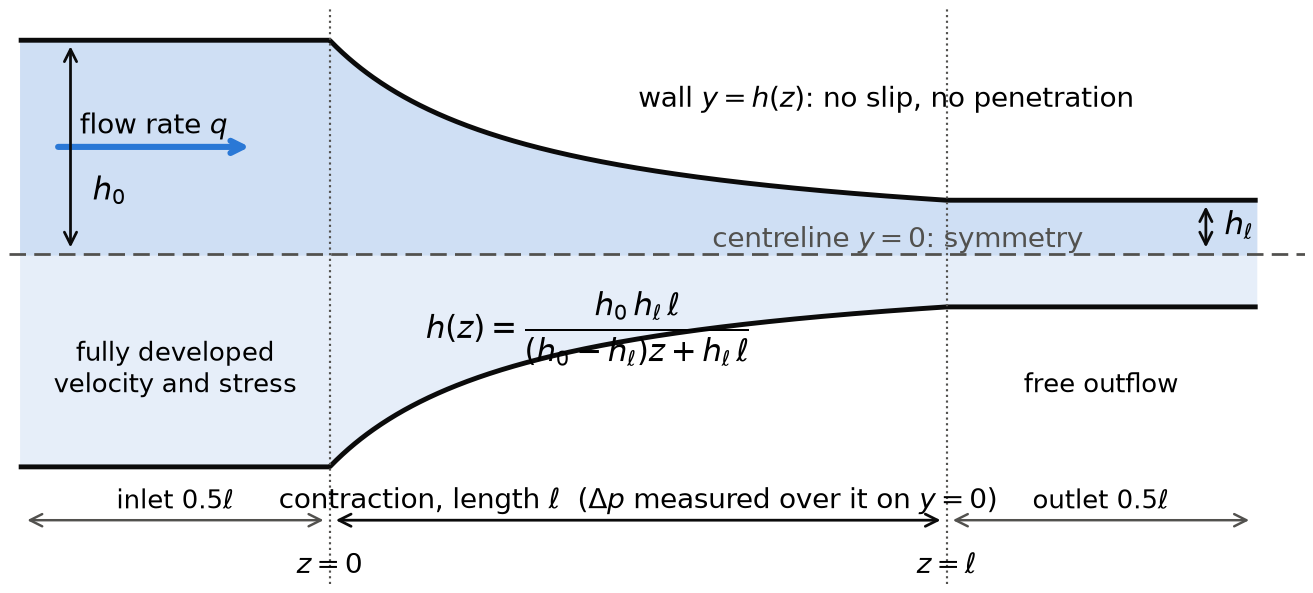
\includegraphics[width=0.86\linewidth]{r01_geometry.png}
\caption{Sketch of the problem (drawn to the scale of the hyperbolic contraction, with the height exaggerated: the real channel is $1/\epsilon=50$ or $10$ times longer than the outlet half-height). The shaded upper half is the computational domain. Boundary conditions: no slip and no penetration on the wall, symmetry on the centreline, fully developed velocity and polymer stress at the inlet, free outflow.}
\label{fig:geom}
\end{figure}

\subsection{Governing equations}
The flow is steady, incompressible and inertia-free (the Reynolds number is below $3\times10^{-6}$, table~\ref{tab:params}). Mass and momentum conservation read
\begin{align}
\nabla\cdot\mathbf{u}&=0, \label{eq:mass}\\
\mathbf{0}&=-\nabla p+\eta_s\nabla^2\mathbf{u}+\nabla\cdot\boldsymbol{\tau}_p, \label{eq:mom}
\end{align}
where $\eta_s$ is the solvent viscosity and $\boldsymbol\tau_p$ the polymer stress. In the Oldroyd-B model \cite{oldroyd1950,bird1987} the polymer stress follows from a conformation tensor $\mathbf{A}$, which measures the average stretch and orientation of the polymer molecules ($\mathbf{A}=\mathbf{I}$ at rest):
\begin{equation}
\boldsymbol\tau_p=\frac{\eta_p}{\lambda}\,(\mathbf{A}-\mathbf{I}),\qquad
\mathbf{A}+\lambda\left[\mathbf{u}\cdot\nabla\mathbf{A}-(\nabla\mathbf{u})^{\mathrm T}\cdot\mathbf{A}-\mathbf{A}\cdot\nabla\mathbf{u}\right]=\mathbf{I}.
\label{eq:oldroyd}
\end{equation}
Here $\eta_p$ is the polymer viscosity and $\lambda$ the relaxation time; $\eta_0=\eta_s+\eta_p$ is the zero-shear viscosity. The bracket is the upper-convected derivative: the conformation is carried with the flow and stretched by the velocity gradient, and it relaxes to $\mathbf I$ over the time $\lambda$.

\subsection{Scaling}
Following the article \cite{boyko2022}, every quantity is scaled by its natural size in a narrow channel, so that all terms are of order one. With $u_c=q/(2h_\ell)$, $\epsilon=h_\ell/\ell$ and $p_c=\eta_0u_c\ell/h_\ell^2$,
\begin{equation}
Z=\frac{z}{\ell},\quad Y=\frac{y}{h_\ell},\quad U_z=\frac{u_z}{u_c},\quad U_y=\frac{u_y}{\epsilon u_c},\quad P=\frac{p}{p_c},\quad H(Z)=\frac{h}{h_\ell}=\frac{\alpha}{(\alpha-1)Z+1}.
\label{eq:scales}
\end{equation}
The polymer stress is scaled with $p_c$ (axial normal stress), $\eta_0u_c/h_\ell$ (shear stress) and $\eta_0u_c/\ell$ (transverse normal stress). The corresponding scaled conformation $\tilde{\mathbf A}$ is
\begin{equation}
\tilde A_{zz}=\frac{\epsilon^2}{\De}\,(A_{zz}-1),\qquad
\tilde A_{yz}=\frac{\epsilon}{\De}\,A_{yz},\qquad
\tilde A_{yy}=\frac{1}{\De}\,(A_{yy}-1),\qquad
\mathbf T=\bt\,\tilde{\mathbf A},
\label{eq:Ascale}
\end{equation}
where $\mathbf T$ is the scaled polymer stress. Three dimensionless groups appear:
\begin{equation}
\De=\frac{\lambda u_c}{\ell},\qquad \epsilon=\frac{h_\ell}{\ell},\qquad \bt=\frac{\eta_p}{\eta_0}.
\label{eq:groups}
\end{equation}
The Deborah number compares the polymer memory with the time the liquid spends in the contraction; $\bt$ is the share of the viscosity contributed by the polymer.

\subsection{Scaled equations}
Substituting (\ref{eq:scales})--(\ref{eq:Ascale}) into (\ref{eq:mass})--(\ref{eq:oldroyd}) gives, without further approximation,
\begin{align}
&\frac{\partial U_z}{\partial Z}+\frac{\partial U_y}{\partial Y}=0, \label{eq:s_mass}\\
&\frac{\partial P}{\partial Z}=(1-\bt)\left(\epsilon^2\frac{\partial^2U_z}{\partial Z^2}+\frac{\partial^2U_z}{\partial Y^2}\right)+\bt\left(\frac{\partial\tilde A_{zz}}{\partial Z}+\frac{\partial\tilde A_{yz}}{\partial Y}\right), \label{eq:s_zmom}\\
&\frac{\partial P}{\partial Y}=\epsilon^2\left[(1-\bt)\left(\epsilon^2\frac{\partial^2U_y}{\partial Z^2}+\frac{\partial^2U_y}{\partial Y^2}\right)+\bt\left(\frac{\partial\tilde A_{yz}}{\partial Z}+\frac{\partial\tilde A_{yy}}{\partial Y}\right)\right], \label{eq:s_ymom}\\
&\De\left(\mathbf U\cdot\nabla\tilde A_{zz}-2\frac{\partial U_z}{\partial Z}\tilde A_{zz}-2\frac{\partial U_z}{\partial Y}\tilde A_{yz}\right)-2\epsilon^2\frac{\partial U_z}{\partial Z}=-\tilde A_{zz}, \label{eq:s_azz}\\
&\De\left(\mathbf U\cdot\nabla\tilde A_{yy}-2\frac{\partial U_y}{\partial Z}\tilde A_{yz}-2\frac{\partial U_y}{\partial Y}\tilde A_{yy}\right)-2\frac{\partial U_y}{\partial Y}=-\tilde A_{yy}, \label{eq:s_ayy}\\
&\De\left(\mathbf U\cdot\nabla\tilde A_{yz}-\frac{\partial U_y}{\partial Z}\tilde A_{zz}-\frac{\partial U_z}{\partial Y}\tilde A_{yy}\right)-\epsilon^2\frac{\partial U_y}{\partial Z}-\frac{\partial U_z}{\partial Y}=-\tilde A_{yz}, \label{eq:s_ayz}
\end{align}
with $\mathbf U\cdot\nabla=U_z\,\partial_Z+U_y\,\partial_Y$. Setting $\epsilon=0$ gives the lubrication limit, in which the pressure is uniform across the channel; keeping $\epsilon$ gives the full two-dimensional Stokes--Oldroyd-B problem. Both are solved in this work.

\subsection{Boundary conditions}
\begin{align}
&\text{wall } Y=H(Z): && U_z=U_y=0, \label{eq:bc_wall}\\
&\text{centreline } Y=0: && \partial_YU_z=0,\ U_y=0,\ \partial_Y\tilde A_{zz}=\partial_Y\tilde A_{yy}=0,\ \tilde A_{yz}=0, \label{eq:bc_sym}\\
&\text{flow rate:} && \int_0^{H(Z)}U_z\,\mathrm dY=1\quad\text{at every }Z, \label{eq:bc_flux}\\
&\text{inlet } Z=Z_{\mathrm{in}}=-0.5: && U_z=\tfrac32\,\frac{H^2-Y^2}{H^3},\ U_y=0,\ \tilde A_{zz}=\frac{18\,\De\,Y^2}{H^6},\ \tilde A_{yz}=-\frac{3Y}{H^3},\ \tilde A_{yy}=0, \label{eq:bc_in}\\
&\text{outlet } Z=1.5: && \text{fully developed velocity; no condition on }\tilde{\mathbf A}\text{ (it is carried out by the flow)}. \label{eq:bc_out}
\end{align}
The inlet stress (\ref{eq:bc_in}) is the exact fully developed Oldroyd-B solution in the straight inlet ($H=\alpha$). The pressure is fixed only up to a constant, and the quantity of interest is the centreline pressure drop across the contraction,
\begin{equation}
\Delta P=P(0,0)-P(1,0),\qquad \Delta p=p_c\,\Delta P.
\label{eq:dP}
\end{equation}

\subsection{Where the pressure drop comes from}
Integrating the $z$-momentum equation (\ref{eq:s_zmom}) along the centreline from $Z=1$ to $Z=0$ splits $\Delta P$ into four parts. Writing the polymer stress as a viscous part plus an elastic excess, $\De\,S_{zz}=\tilde A_{zz}-2\epsilon^2\partial_ZU_z$ and $\De\,S_{yz}=\tilde A_{yz}-\epsilon^2\partial_ZU_y-\partial_YU_z$, gives
\begin{equation}
\Delta P=\underbrace{\epsilon^2\Big[\frac{\partial U_z}{\partial Z}\Big]_{1}^{0}}_{\term{1}}
+\underbrace{\int_1^0\frac{\partial^2U_z}{\partial Y^2}\,\mathrm dZ}_{\term{2}}
+\underbrace{\bt\,\De\,\big[S_{zz}\big]_{1}^{0}}_{\term{3}}
+\underbrace{\bt\,\De\int_1^0\frac{\partial S_{yz}}{\partial Y}\,\mathrm dZ}_{\term{4}},
\qquad\text{all at }Y=0,
\label{eq:terms}
\end{equation}
which is the decomposition used in the article \cite{boyko2022}. Terms \term{1} and \term{2} are viscous (with the total viscosity $\eta_0$); \term{3} is the elastic axial normal stress; \term{4} is the gradient of the elastic shear stress. The PINN gives $\Delta P$ in two independent ways: directly from the pressure, by (\ref{eq:dP}), and from the sum (\ref{eq:terms}). Their agreement is a check on the solution.

\section{Numerical analysis}

\subsection{Parameters}
Table~\ref{tab:params} lists the physical parameters of the two channels studied in the article \cite{boyko2022}, which are used unchanged here, together with the derived groups. Since $\ell/u_c=1$\,s, the relaxation time in seconds equals the Deborah number. All computations use the scaled equations, so only $\alpha$, $\bt$, $\epsilon$ and $\De$ enter; dimensional pressure drops follow from $\Delta p=p_c\Delta P$.

\begin{table}[H]
\centering\small
\caption{Physical parameters (from \cite{boyko2022}) and derived quantities.}
\label{tab:params}
\begin{tabular}{@{}llll@{}}
\toprule
Quantity & Symbol & Case I & Case II\\
\midrule
contraction length & $\ell$ & 5 mm & 5 mm\\
inlet / outlet half-height & $h_0$, $h_\ell$ & 0.4 mm, 0.1 mm & 2 mm, 0.5 mm\\
contraction ratio & $\alpha=h_0/h_\ell$ & 4 & 4\\
aspect ratio & $\epsilon=h_\ell/\ell$ & 0.02 & 0.1\\
flow rate per unit width & $q$ & $10^{-6}$ m$^2$\,s$^{-1}$ & $5\times10^{-6}$ m$^2$\,s$^{-1}$\\
characteristic velocity & $u_c=q/(2h_\ell)$ & 5 mm\,s$^{-1}$ & 5 mm\,s$^{-1}$\\
zero-shear, solvent, polymer viscosity & $\eta_0$, $\eta_s$, $\eta_p$ & 1, 0.6, 0.4 Pa\,s & 1, 0.6, 0.4 Pa\,s\\
viscosity ratio & $\bt=\eta_p/\eta_0$ & 0.4 & 0.4\\
density & $\rho$ & 1 kg\,m$^{-3}$ & 1 kg\,m$^{-3}$\\
relaxation time & $\lambda$ & 0--0.3 s & 0--0.3 s\\
Deborah number & $\De=\lambda u_c/\ell$ & 0--0.3 & 0--0.3\\
Weissenberg number & $\mathrm{Wi}=\De/\epsilon$ & 0--15 & 0--3\\
Reynolds number & $\mathrm{Re}=\rho u_ch_\ell/\eta_0$ & $5\times10^{-7}$ & $2.5\times10^{-6}$\\
characteristic pressure & $p_c=\eta_0u_c\ell/h_\ell^2$ & 2500 Pa & 100 Pa\\
\bottomrule
\end{tabular}
\end{table}

\subsection{Three independent routes to the solution}
Three methods were implemented, so that each result could be checked against at least one other.
\begin{enumerate}[label=(\alph*)]
\item \textbf{Low-$\De$ perturbation theory, re-derived.} The expansion $\mathbf U=\mathbf U_0+\De\,\mathbf U_1+\dots$ of (\ref{eq:s_mass})--(\ref{eq:s_ayz}) at $\epsilon=0$ was carried out symbolically for a general shape $H(Z)$ with SymPy \cite{meurer2017}, and the third-order pressure drop was obtained directly from the $O(\De^3)$ momentum balance, without the reciprocal theorem. For $\alpha=4$, $\bt=0.4$ this gives
\begin{equation}
\Delta P\approx \sum_{n=0}^{3}\De^n\,\Delta P_n
=0.996094-1.792969\,\De+5.532589\,\De^2-14.661362\,\De^3,
\label{eq:series}
\end{equation}
where $\Delta P_0=3\int_0^1H^{-3}\mathrm dZ=255/256$ and $\Delta P_1=\tfrac92\bt\,(H(0)^{-4}-H(1)^{-4})$. The same symbolic tools gave the Newtonian correction for finite $\epsilon$ (extended lubrication theory, cf.\ \cite{tavakol2017}),
\begin{equation}
\Delta P_{\De=0}=\frac{255}{256}+\epsilon^2\!\int_0^1\!\frac{3\,(14H'^2-HH'')}{10\,H^3}\,\mathrm dZ+O(\epsilon^4)=\frac{255}{256}+3.743\,\epsilon^2+O(\epsilon^4).
\label{eq:eps2}
\end{equation}

\item \textbf{Reference solver for the lubrication limit ($\epsilon\to0$).} Equations (\ref{eq:s_mass})--(\ref{eq:s_ayz}) with $\epsilon=0$ are discretised on the mapped coordinate $\eta=Y/H(Z)\in[0,1]$ with Chebyshev points across the channel \cite{trefethen2000} (20 intervals, clustered at the wall) and finite differences along it (second-order upwind for stress advection, second-order central for the velocity derivatives; $\Delta Z=1.5\times10^{-3}$ near the two corners and $5\times10^{-3}$ elsewhere). $U_y$ is obtained from a stream function, so mass is conserved exactly. All stations are solved \emph{at once} by Newton's method, with a sparse Jacobian built by coloured finite differences \cite{curtis1974} and continuation in $\De$; the tolerance is $10^{-8}$ and one $\De$ takes about 5\,s. A simpler station-by-station march down the channel was tried first and diverged for every $\De>0$, faster on finer grids: the axial-stress gradient $\partial_Z\tilde A_{zz}$ changes the velocity, and $\partial_ZU_z$ in turn changes $\tilde A_{zz}$, so the problem needs information from downstream and is ill-posed as an initial-value problem. Table~\ref{tab:conv} shows that the result is independent of the grid, the corner rounding and the outlet length to four digits.

\item \textbf{Physics-informed neural network} (section~\ref{sec:pinn}), for $\epsilon=0$, $0.02$ and $0.1$.
\end{enumerate}

\begin{table}[H]
\centering\small
\caption{Convergence of the reference solver: $\Delta P$ for $\epsilon\to0$. $N$: Chebyshev intervals across the channel; $\delta$: corner rounding half-width; $L_{\mathrm{out}}$: outlet length.}
\label{tab:conv}
\footnotesize
\begin{tabular}{@{}lccc@{}}
\toprule
Case & $\De=0.1$ & $\De=0.2$ & $\De=0.3$\\
\midrule
base: $N=20$, $\Delta Z=5\times10^{-3}$ ($1.5\times10^{-3}$ at corners), $\delta=0.01$, $L_{\mathrm{out}}=0.5$ & 0.86085 & 0.78195 & 0.73284\\
$N=28$ (finer across) & 0.86085 & 0.78195 & 0.73285\\
$\Delta Z$ halved (finer along) & 0.86083 & 0.78193 & 0.73281\\
$\delta=0.005$ (sharper corners) & 0.86081 & 0.78188 & 0.73275\\
$\delta=0.02$ (rounder corners) & 0.86089 & 0.78202 & 0.73292\\
$L_{\mathrm{out}}=1.0$ (longer outlet) & 0.86085 & 0.78195 & 0.73284\\
\bottomrule
\end{tabular}
\end{table}

\subsection{The physics-informed neural network}
\label{sec:pinn}
\textbf{Exact constraints.} The domain $-0.5\le Z\le1.5$, $0\le\eta\le1$ is mapped so that the wall is the fixed line $\eta=1$. The velocity is built from a stream function,
\begin{equation}
\Psi=\tfrac12(3\eta-\eta^3)+\eta\,(1-\eta^2)^2\,B(Z)\,c\,N_\psi(Z,\eta^2),\qquad U_z=\frac{\partial\Psi}{\partial Y},\quad U_y=-\frac{\partial\Psi}{\partial Z},
\label{eq:psi}
\end{equation}
where $N_\psi$ is a neural network, $c=0.1$, and $B(Z)=\big(1-e^{-(Z-Z_{\mathrm{in}})/0.1}\big)\big(1-e^{-(Z_{\mathrm{out}}-Z)/0.1}\big)$ vanishes at both ends of the domain ($Z_{\mathrm{in}}=-0.5$, $Z_{\mathrm{out}}=1.5$). For \emph{any} network weights, (\ref{eq:psi}) satisfies mass conservation (\ref{eq:s_mass}), the wall and symmetry conditions (\ref{eq:bc_wall})--(\ref{eq:bc_sym}), the flow rate (\ref{eq:bc_flux}) and the fully developed inflow and outflow. Feeding the networks $\eta^2$ instead of $\eta$ makes every output even in $\eta$, so the symmetry is built in. The pressure and the conformation are
\begin{equation}
P=N_P(Z)+\epsilon^2N_{P1}(Z,\eta^2),\qquad
\tilde A_{ij}=\tilde A_{ij}^{\mathrm{in}}(\eta)+R(Z)\,s_{ij}(Z)\,N_{ij}(Z,\eta^2),
\label{eq:PA}
\end{equation}
with $R(Z)=1-e^{-(Z-Z_{\mathrm{in}})/0.1}$ vanishing at the inlet, so that the inflow stress (\ref{eq:bc_in}) holds exactly, and with the local stress sizes $s_{zz}=18\max(\De,0.05)/H^4$, $s_{yz}=3\eta/H^2$ (which also makes $\tilde A_{yz}$ odd in $\eta$) and $s_{yy}=3(\alpha-1)/\alpha$. These sizes keep the network outputs of order one along a channel whose stresses vary 256-fold. The pressure split in (\ref{eq:PA}) makes $P$ exactly uniform across the channel when $\epsilon=0$, as the scaling requires.

\textbf{Networks and inputs.} Each field ($\Psi$, $P$, $P_1$, $\tilde A_{zz}$, $\tilde A_{yy}$, $\tilde A_{yz}$) has its own fully connected network with 4 hidden layers of 64 $\tanh$ neurons. The inputs, scaled to $[-1,1]$, are $Z$, $\eta^2$, $H(Z)$ and an indicator of the contraction section. One further network takes $\De$ as an extra input (80 neurons per layer) and covers $0\le\De\le0.3$ at $\epsilon=0.02$ with a single set of weights. The two corners where the straight sections meet the hyperbola are rounded over a half-width $\delta=0.01$ ($\epsilon=0$) or $0.03$ ($\epsilon>0$); table~\ref{tab:conv} shows that this changes $\Delta P$ by less than $0.03\,\%$.

\textbf{Loss.} With all boundary conditions exact, the loss contains only the residuals $r_k$ of (\ref{eq:s_zmom})--(\ref{eq:s_ayz}), each divided by its local size $n_k$:
\begin{equation}
\begin{gathered}
\mathcal L=\sum_{k}\frac1{N_c}\sum_{i=1}^{N_c}\left(\frac{r_k(Z_i,Y_i)}{n_k(Z_i)}\right)^2,\\
n_z=\frac{3}{H^3},\quad n_{zz}=\frac{18\max(\De,0.05)}{H^4},\quad n_{yz}=\frac{3}{H^2},\quad n_{yy}=\frac{3(\alpha-1)}{\alpha},\quad n_y=\frac{3}{H^2},
\end{gathered}
\label{eq:loss}
\end{equation}
where the $y$-momentum residual (divided by $\epsilon^2$) is included only for $\epsilon>0$. For $\epsilon>0$ no $n_k$ is allowed below $10\,\%$ of its outlet value, which stops the tiny pressure gradient in the wide inlet from inflating the residuals there. There are therefore no loss weights to tune.

\textbf{Collocation points and training.} $N_c=4096$ random points per step (6144 for the cold-started runs at $\epsilon=0.02$) are redrawn every 50 steps: 45\,\% in the contraction, 20\,\% clustered towards the outlet where the stresses are largest, 10\,\% near the two corners, the rest in the straight sections, and 30\,\% of all points clustered near the wall. Training uses Adam \cite{kingma2015} for 6000 steps with the learning rate decaying exponentially from $2\times10^{-3}$ to $2\times10^{-5}$, followed by 1500 steps of L-BFGS \cite{liu1989} in double precision on 8192--12288 fresh points. Higher $\De$ are reached by continuation: each run starts from the converged weights at the previous $\De$, with 2000--3000 Adam steps from a learning rate of $5\times10^{-4}$, followed by 1500 L-BFGS steps ($\epsilon=0$) or three L-BFGS rounds of 900 steps, each on fresh points ($\epsilon>0$; also used for the cold-started $\epsilon>0$ runs). Sixteen networks were trained: seven at $\epsilon=0$ ($\De=0$, 0.05, \dots, 0.3), four each at $\epsilon=0.02$ and 0.1 ($\De=0$, 0.1, 0.2, 0.3), and the $\De$-input network.

\textbf{Pressure drop.} $\Delta P$ is evaluated from (\ref{eq:dP}) and, independently, from (\ref{eq:terms}) with 400-point Gauss--Legendre quadrature.

\subsection{Code and hardware}
All code is written in Python with PyTorch \cite{paszke2019}, NumPy, SciPy, SymPy and Matplotlib and is organised as a package plus scripts:
\begin{center}\small
\begin{tabularx}{\linewidth}{@{}lX@{}}
\toprule
File & Content\\
\midrule
\code{03\_code/oldroydb/geometry.py} & channel shape (\ref{eq:hz}) with straight sections and rounded corners\\
\code{03\_code/oldroydb/analytical.py} & perturbation results (\ref{eq:series})\\
\code{03\_code/oldroydb/lubrication\_fd.py} & reference solver (global Newton, Chebyshev $\times$ finite differences)\\
\code{03\_code/oldroydb/pinn.py} & PINN: constrained outputs (\ref{eq:psi})--(\ref{eq:PA}), residuals, loss (\ref{eq:loss}), training, $\Delta P$ both ways\\
\code{03\_code/oldroydb/compare.py}, \code{report.py} & error measures, tables and figures\\
\code{03\_code/scripts/} & SymPy derivation, reference runs, training campaign, summaries\\
\code{06\_submission/report/make\_report\_figures.py} & every figure of this report, from the saved results\\
\code{gui.py}, \code{predict.py} & explorer window and command-line predictor using the trained networks\\
\bottomrule
\end{tabularx}
\end{center}
A one-command script (\code{setup\_and\_run.bat} on Windows, \code{setup\_and\_run.sh} on macOS/Linux) installs everything in a private environment and runs a check, the notebook or the explorer; it was tested on clean Windows and macOS machines (GitHub Actions, Python 3.12 and 3.14). Training used one Apple M4 laptop (CPU in double precision; the Apple GPU in single precision for $\epsilon=0.1$) and took 7--55 minutes per network, 4.8 hours in total.

\section{Results and discussion}
Every figure and table in this section is computed by the code of this work. The curves labelled ``low-De theory'' are my evaluation of the re-derived series (\ref{eq:series}).

\subsection{Training}
Figure~\ref{fig:loss} shows a typical training history, for a network warm-started from the converged solution at the previous $\De$. At the first step the $z$-momentum residual is large ($0.17$), because the stresses of the old solution no longer balance the pressure at the new $\De$; within 250 Adam steps it falls by almost three orders of magnitude, and all residuals then decrease slowly together, as intended when each is divided by its own size. Adam ends at a total loss of $1.3\times10^{-3}$. L-BFGS, with fresh points, lowers it by a further factor of 3.4 to $3.7\times10^{-4}$. The small jump when L-BFGS starts is the effect of the new points: it shows how much of the loss was specific to the old points, and it is small. Table~\ref{tab:cost} confirms this for every network: the loss on fresh points never used in training is 7--50\,\% (typically 10--25\,\%) above the training loss, so none of the networks overfits. The $\epsilon=0.1$ networks end with a higher loss ($\sim2\times10^{-3}$) because the Apple GPU only offers single precision for L-BFGS.

\begin{figure}[H]
\centering
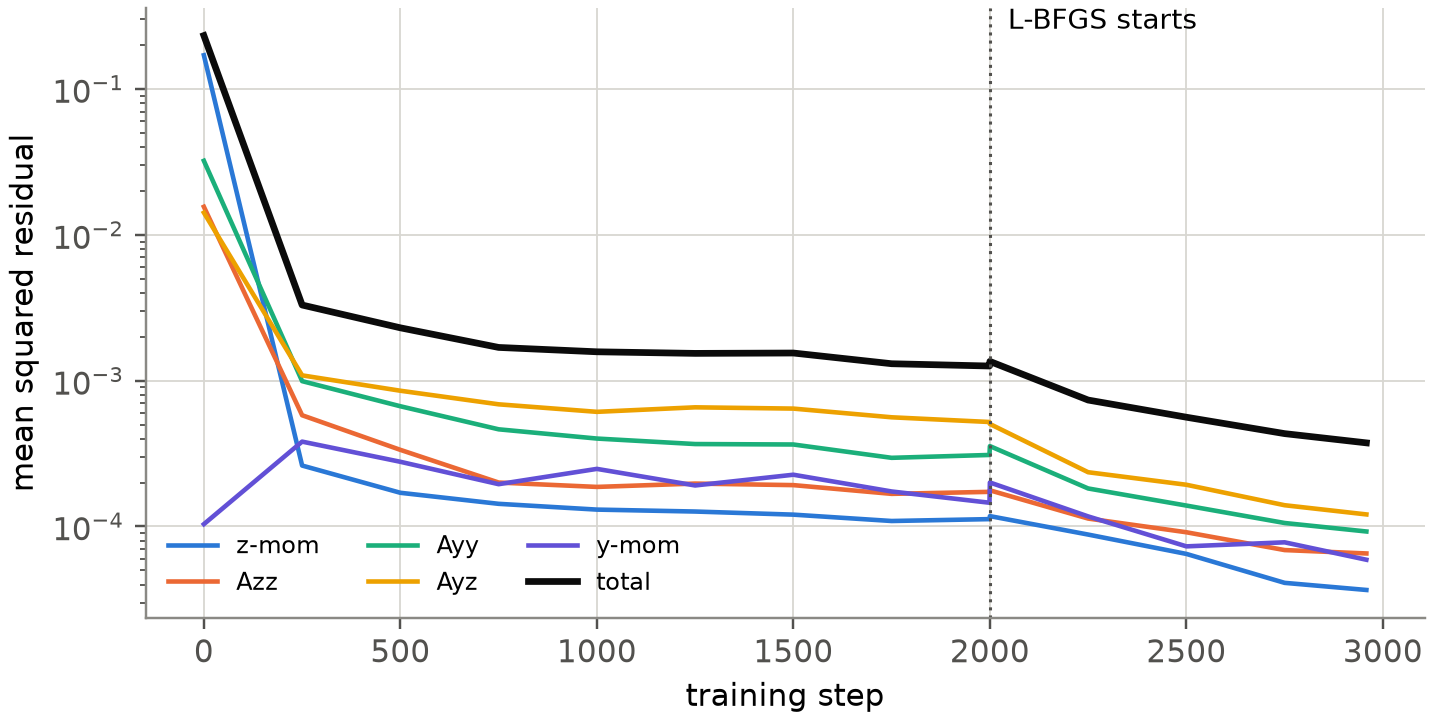
\includegraphics[width=0.72\linewidth]{r02_loss_eps002_De02.png}
\caption{Training history of the PINN at $\epsilon=0.02$, $\De=0.2$ (warm-started from $\De=0.1$): mean squared normalised residual of each equation and the total, against training step. The dotted line marks the switch from Adam to L-BFGS.}
\label{fig:loss}
\end{figure}

\begin{table}[H]
\centering\small
\caption{Training cost and final loss of every network (Apple M4 laptop). Held-out loss: on 8192--12288 fresh points never used in training.}
\label{tab:cost}
\footnotesize\setlength{\tabcolsep}{4pt}
\begin{tabular}{@{}llccc@{}}
\toprule
$\epsilon$ & $\De$ & minutes & final loss & held-out loss\\
\midrule
0 & 0, 0.05, \dots, 0.30 (7 runs) & 18, 17, 14, 15, 18, 7, 8 & $1.9\times10^{-5}$--$9.9\times10^{-5}$ & $2.8\times10^{-5}$--$1.2\times10^{-4}$\\
0.02 & 0, 0.1, 0.2, 0.3 & 49, 14, 15, 12 & $9.1\times10^{-5}$--$5.0\times10^{-4}$ & $9.7\times10^{-5}$--$5.8\times10^{-4}$\\
0.1 & 0, 0.1, 0.2, 0.3 (single precision) & 24, 7, 7, 8 & $1.8$--$2.0\times10^{-3}$ & $2.1$--$2.3\times10^{-3}$\\
0.02 & 0--0.3 ($\De$ as input) & 55 & $2.1\times10^{-4}$ & $2.7\times10^{-4}$\\
\bottomrule
\end{tabular}
\end{table}

\subsection{Pressure drop in the lubrication limit}
Figure~\ref{fig:dplub} and table~\ref{tab:dplub} compare the PINN with the reference solver and the series for $\epsilon=0$. The pressure drop falls monotonically with elasticity, from 0.996 at $\De=0$ to 0.733 at $\De=0.3$, a reduction of 26\,\%. The PINN follows the reference solver within 0.22\,\% at every $\De$ when $\Delta P$ is taken from the pressure itself, and within 0.09\,\% when it is taken from the momentum integral (\ref{eq:terms}); the two PINN routes agree with each other within 0.2\,\%. At $\De=0$ both reproduce $255/256$.

The truncated series behaves very differently. The first-order line falls far too fast, the second-order curve turns upwards, and the third-order curve is accurate only up to $\De\approx0.1$; its error grows to $-1.8\,\%$ at $\De=0.15$, $-5.2\,\%$ at 0.2 and $-23.5\,\%$ at 0.3. The reason is visible in (\ref{eq:series}): the coefficients alternate in sign and grow two- to threefold from one order to the next, so the series behaves roughly like a geometric series with ratio $\approx-3\De$ and cannot be trusted as $\De$ approaches 0.3. The PINN and the reference solver have no such limit, which is the practical value of a numerical solution here.

\begin{figure}[H]
\centering
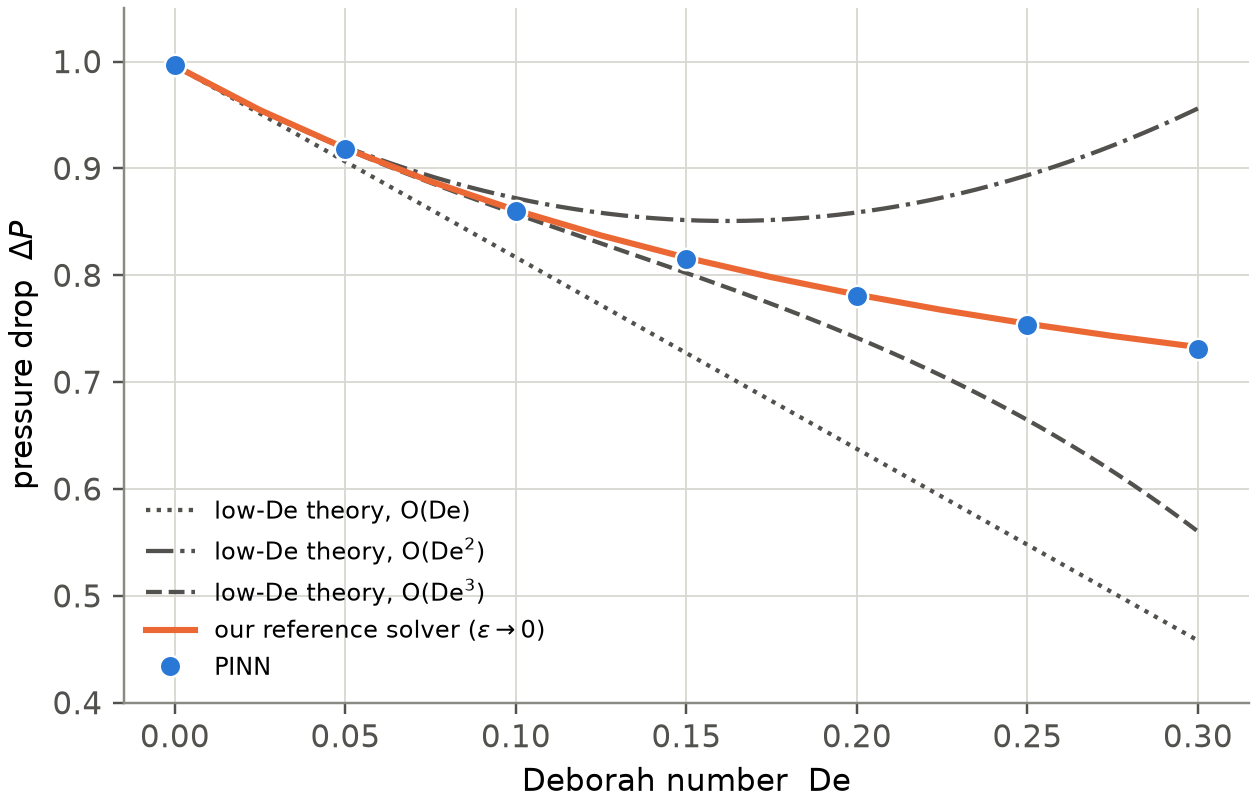
\includegraphics[width=0.62\linewidth]{r03_dp_lubrication.png}
\caption{Scaled pressure drop $\Delta P$ against $\De$ in the lubrication limit ($\epsilon\to0$). Circles: PINN (one network per $\De$). Solid line: reference solver. Dashed and dotted lines: low-$\De$ series (\ref{eq:series}) truncated at first, second and third order.}
\label{fig:dplub}
\end{figure}

\begin{table}[H]
\centering\small
\caption{$\Delta P$ in the lubrication limit. Errors are relative to the reference solver.}
\label{tab:dplub}
\footnotesize\setlength{\tabcolsep}{4pt}
\begin{tabular}{@{}ccccccc@{}}
\toprule
$\De$ & PINN, pressure & PINN, momentum & reference & error (\%) & error, mom.\ (\%) & series $O(\De^3)$ err.\ (\%)\\
\midrule
0.00 & 0.9965 & 0.9964 & 0.9961 & $+0.05$ & $+0.03$ & $0.0$\\
0.05 & 0.9181 & 0.9193 & 0.9188 & $-0.08$ & $+0.06$ & $0.0$\\
0.10 & 0.8599 & 0.8611 & 0.8609 & $-0.11$ & $+0.03$ & $-0.4$\\
0.15 & 0.8151 & 0.8160 & 0.8165 & $-0.17$ & $-0.06$ & $-1.8$\\
0.20 & 0.7802 & 0.7812 & 0.7820 & $-0.22$ & $-0.09$ & $-5.2$\\
0.25 & 0.7534 & 0.7547 & 0.7547 & $-0.17$ & $0.00$ & $-11.9$\\
0.30 & 0.7313 & 0.7327 & 0.7328 & $-0.21$ & $-0.02$ & $-23.5$\\
\bottomrule
\end{tabular}
\end{table}

\subsection{Velocity and stress fields, and where the error sits}
Figure~\ref{fig:fields} compares the PINN fields with the reference solver at the highest elasticity, $\De=0.3$. The axial velocity is nearly parabolic at every station and simply speeds up as the channel narrows; it agrees to 0.2\,\% (relative $L_2$ error over the contraction). The axial polymer stress $T_{zz}$ is positive and confined to a thin layer along the wall that grows towards the outlet, where the stretching is strongest; the shear stress $T_{yz}$ is negative (the wall drags the liquid back) and also largest at the outlet wall. The PINN reproduces these maps with relative errors of 2.1\,\% ($T_{zz}$) and 1.9\,\% ($T_{yz}$). The difference maps (right column) show that the error is not spread over the domain: it is concentrated in a small region at the outlet corner, and to a lesser extent at the inlet corner.

\begin{figure}[H]
\centering
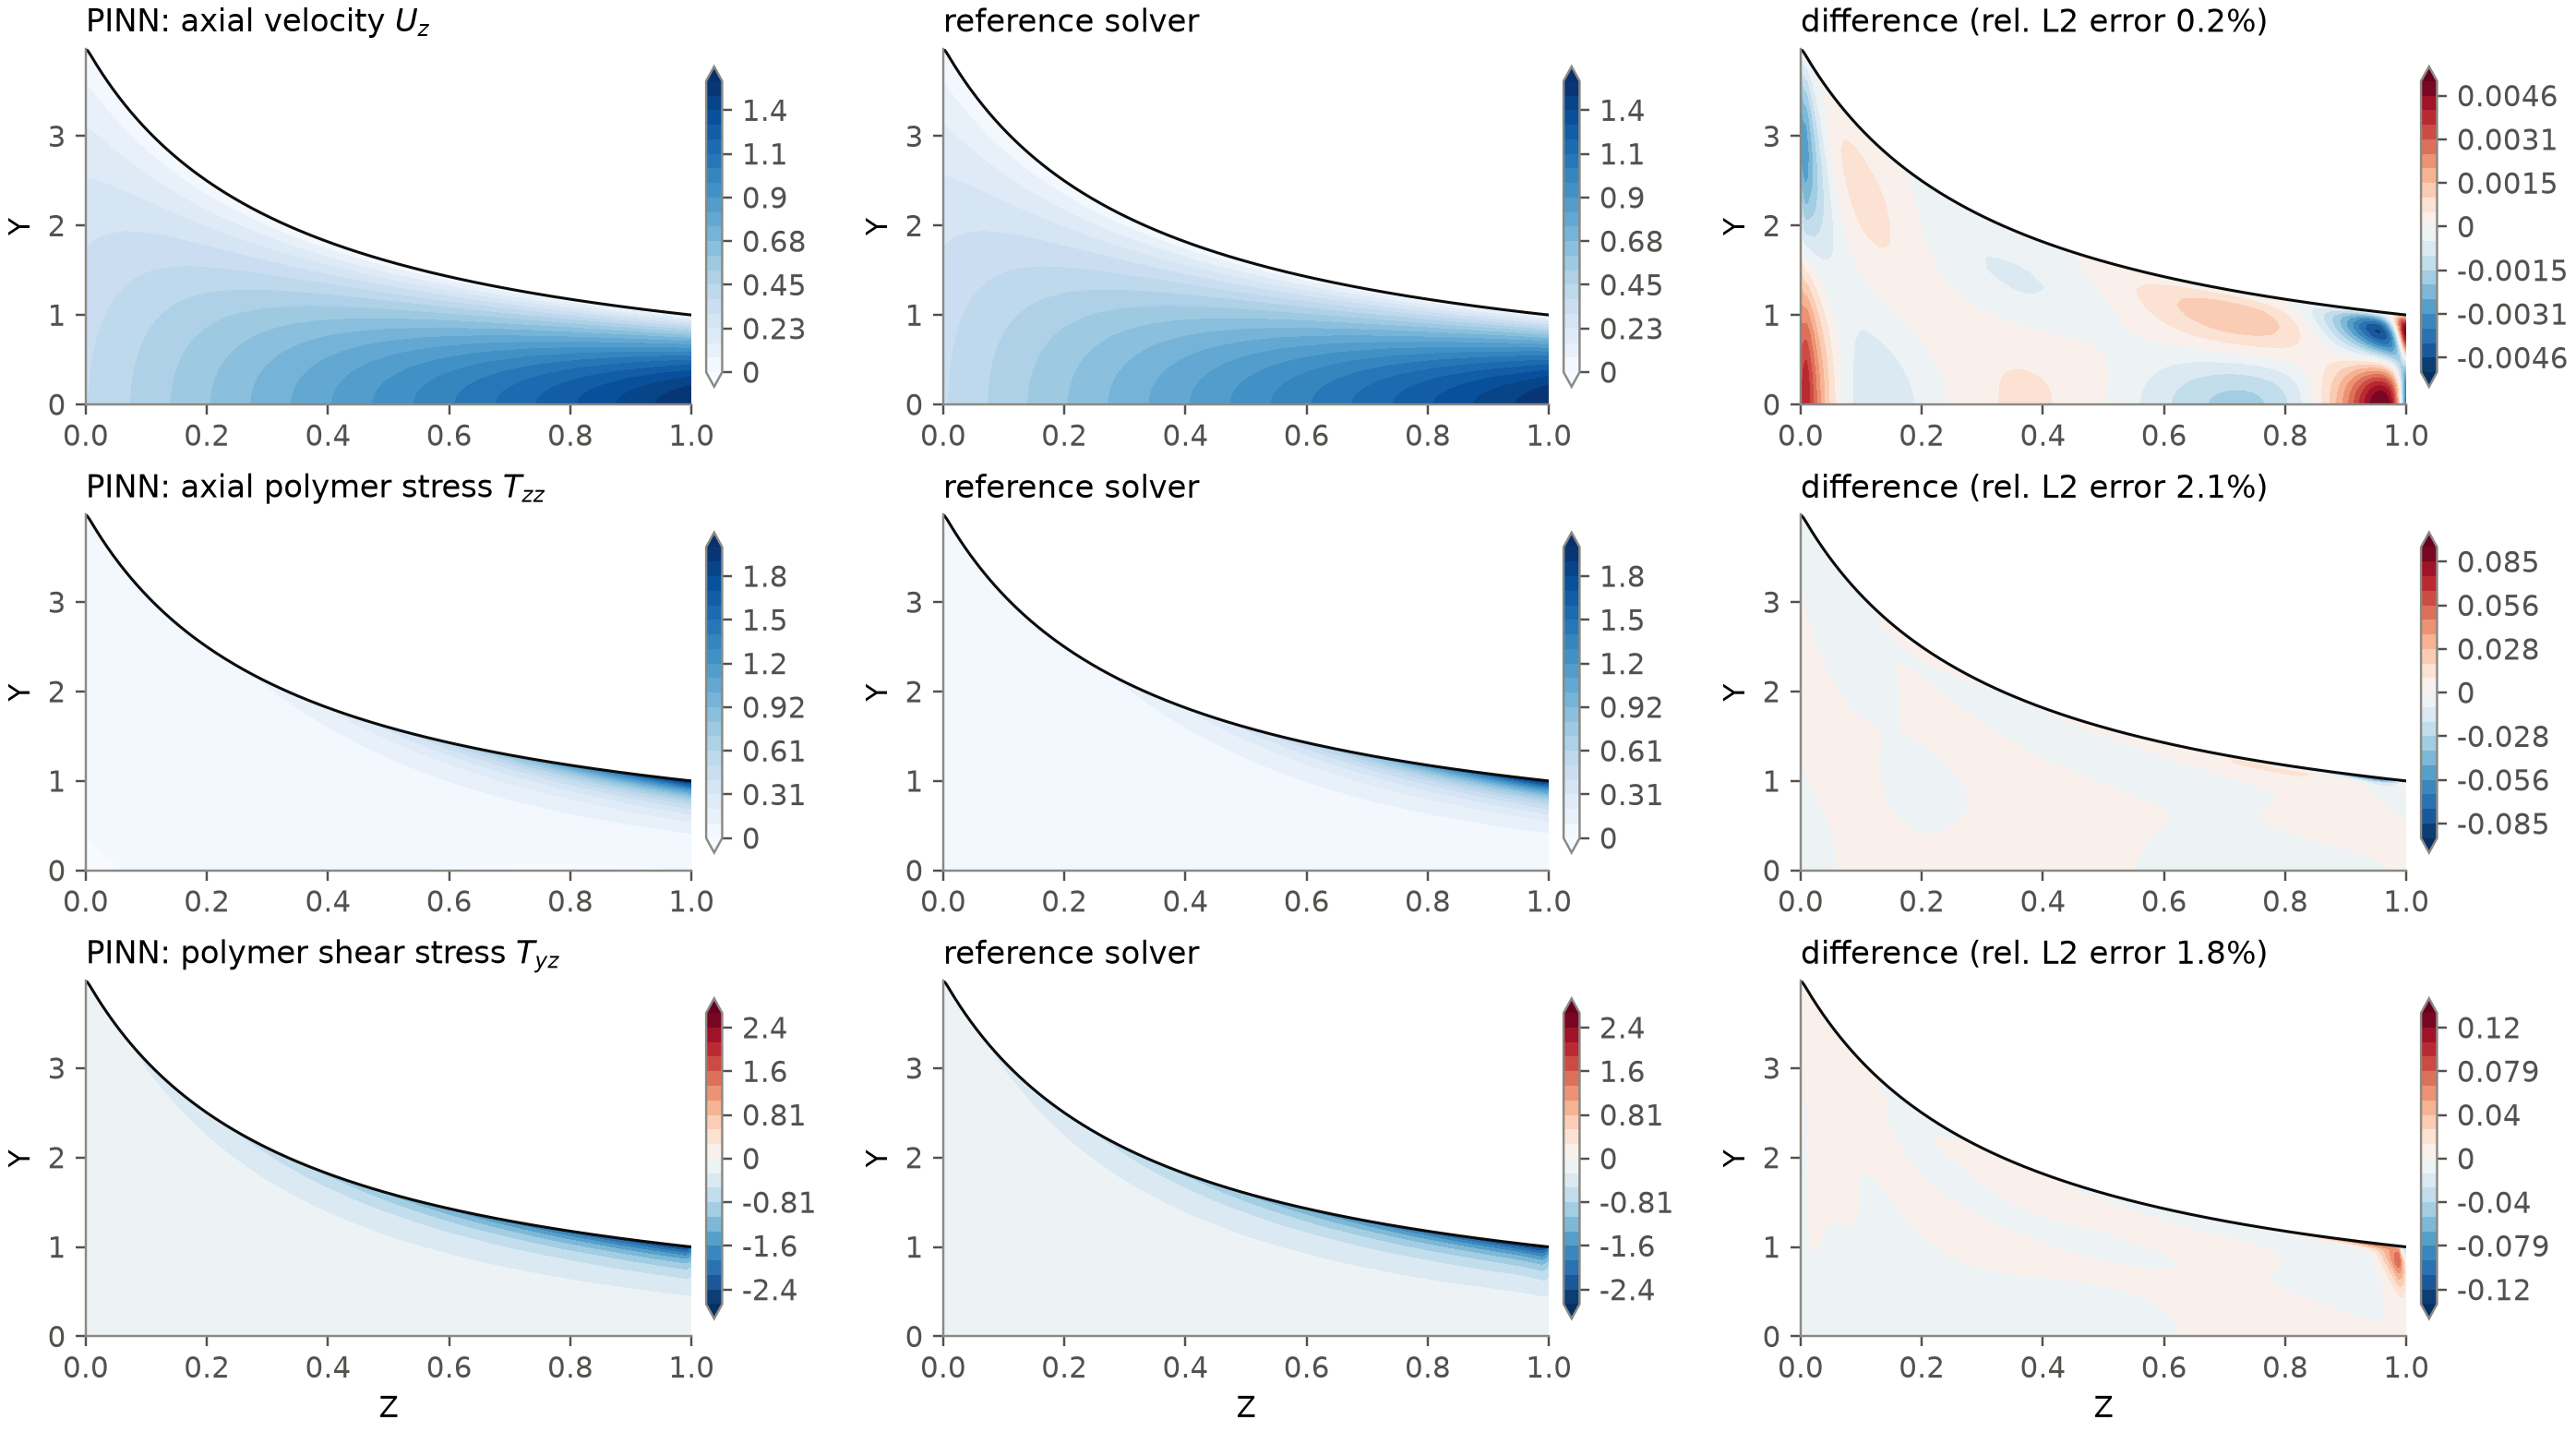
\includegraphics[width=\linewidth]{r04_fields_De03.png}
\caption{Fields at $\De=0.3$, $\epsilon\to0$, over the contraction $0\le Z\le1$. Rows: axial velocity $U_z$, axial polymer stress $T_{zz}$, polymer shear stress $T_{yz}$. Columns: PINN, reference solver, and their difference (with the relative $L_2$ error).}
\label{fig:fields}
\end{figure}

Figure~\ref{fig:erralong} makes this quantitative: it plots, at each station $Z$, the error across the channel divided by the largest size of that field. Away from the two corners the error of every field is between $10^{-4}$ and $5\times10^{-3}$, i.e.\ 0.01--0.5\,\%. It rises to a few percent only in the shaded corner zones, where the wall slope jumps from $H'=0$ to $H'=-12$ (inlet) or from $H'=-0.75$ to 0 (outlet) over 1\,\% of the length. A smooth $\tanh$ network has difficulty representing such a rapid change, and the resulting error is carried downstream by the stress equations. At $\De=0.1$ the errors are about half those at $\De=0.3$. Over all seven $\De$ values the relative $L_2$ errors are 0.02--0.2\,\% for $U_z$, 0.7--2.1\,\% for $T_{zz}$, 0.1--1.9\,\% for $T_{yz}$ and 1--3\,\% for $T_{yy}$; the larger relative error of the small cross-stream velocity $U_y$ (2--5\,\%) also comes from the corners.

\begin{figure}[H]
\centering
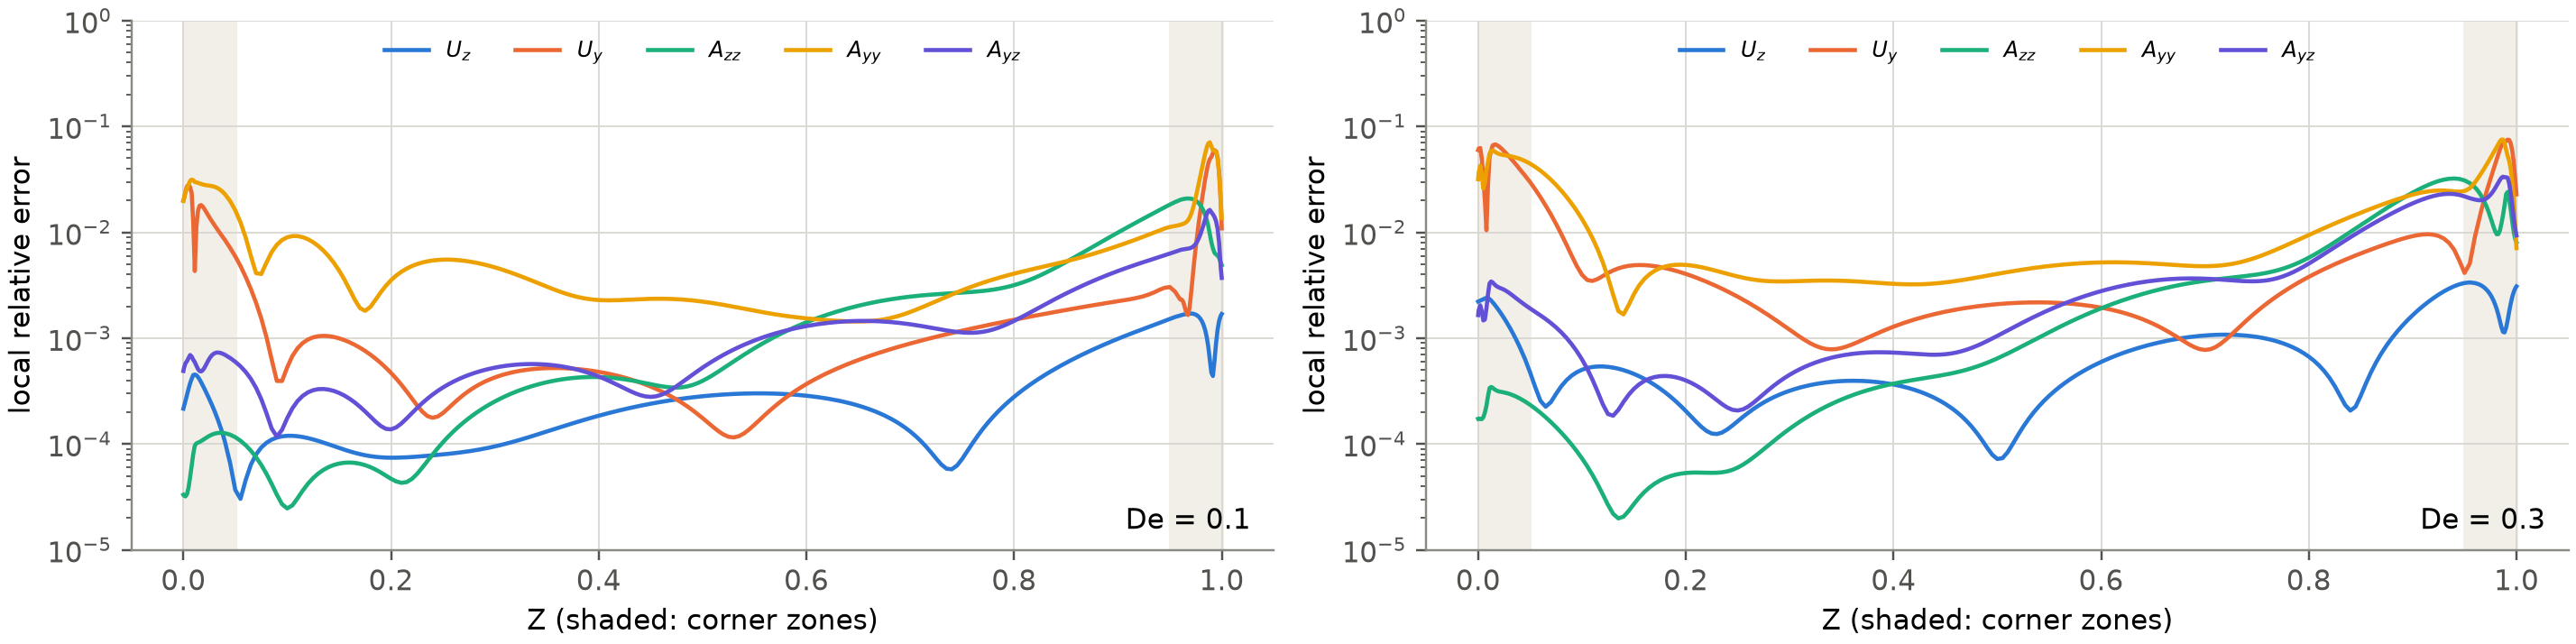
\includegraphics[width=\linewidth]{r05_error_along.png}
\caption{Local error of the PINN along the channel at $\De=0.1$ (left) and $\De=0.3$ (right), $\epsilon\to0$: $L_2$ norm of (PINN $-$ reference) across the channel at each $Z$, divided by the largest such norm of the field. Shaded: the two corner zones.}
\label{fig:erralong}
\end{figure}

\subsection{Full two-dimensional flow at finite aspect ratio}
Figure~\ref{fig:dp2d} shows $\Delta P(\De)$ from the full two-dimensional PINNs for the article's two channels, $\epsilon=0.02$ and $\epsilon=0.1$, together with the lubrication-limit reference solver.

For the slender channel, $\epsilon=0.02$, the PINN pressure drops (0.9968, 0.8600, 0.7776, 0.7252 at $\De=0$, 0.1, 0.2, 0.3) lie within 1.1\,\% of the $\epsilon\to0$ curve. At $\De=0$ the PINN value is 0.08\,\% below the extended-lubrication estimate (\ref{eq:eps2}), $0.99759$, shown by the diamond. The single network with $\De$ as an input (dash-dotted line) traces the whole curve and agrees with the four fixed-$\De$ networks within 0.6\,\% (at $\De=0.3$, 0.7260 against 0.7252); it answers for any intermediate $\De$ in milliseconds without retraining. The two PINN routes to $\Delta P$ (circles and crosses) differ by at most 0.52\,\%.

For the wider channel, $\epsilon=0.1$, the pressure drop is clearly higher than the lubrication value, by 3.1\,\% at $\De=0$ (1.0274) and by 4.0\,\% at $\De=0.3$ (0.7624). This is the effect of the terms of order $\epsilon^2$ in (\ref{eq:s_zmom})--(\ref{eq:s_ayz}): the streamlines curve, the axial velocity varies along the channel and the pressure is no longer uniform across it. The Newtonian estimate (\ref{eq:eps2}) predicts $1.0335$, 0.6\,\% above the PINN; the remaining difference is consistent with the neglected $O(\epsilon^4)$ terms and the corners, which (\ref{eq:eps2}) does not see. The relative reduction of $\Delta P$ by elasticity, $\Delta P(0.3)/\Delta P(0)$, is almost the same for the three aspect ratios (0.736 for $\epsilon\to0$, 0.728 for $\epsilon=0.02$, 0.742 for $\epsilon=0.1$): the geometry sets the Newtonian level, and the elastic reduction is nearly independent of it.

\textbf{Agreement with the article's simulations.} The article reports finite-element pressure drops for these two channels only as a figure \cite[fig.~2]{boyko2022}. I recovered those values from the vector graphics of the PDF for comparison; they are not plotted or tabulated here. Against them, the PINN pressure drops differ by at most 0.68\,\% (pressure route) and 1.05\,\% (momentum route) over both channels and all $\De$, and the reference solver at $\epsilon\to0$ differs from the $\epsilon=0.02$ values by at most 0.37\,\%. In dimensional terms, for case I ($p_c=2500$\,Pa) the PINN gives $\Delta p=2492$\,Pa at $\De=0$ and $1813$\,Pa at $\De=0.3$; for case II ($p_c=100$\,Pa), $102.7$\,Pa and $76.2$\,Pa.

\begin{figure}[H]
\centering
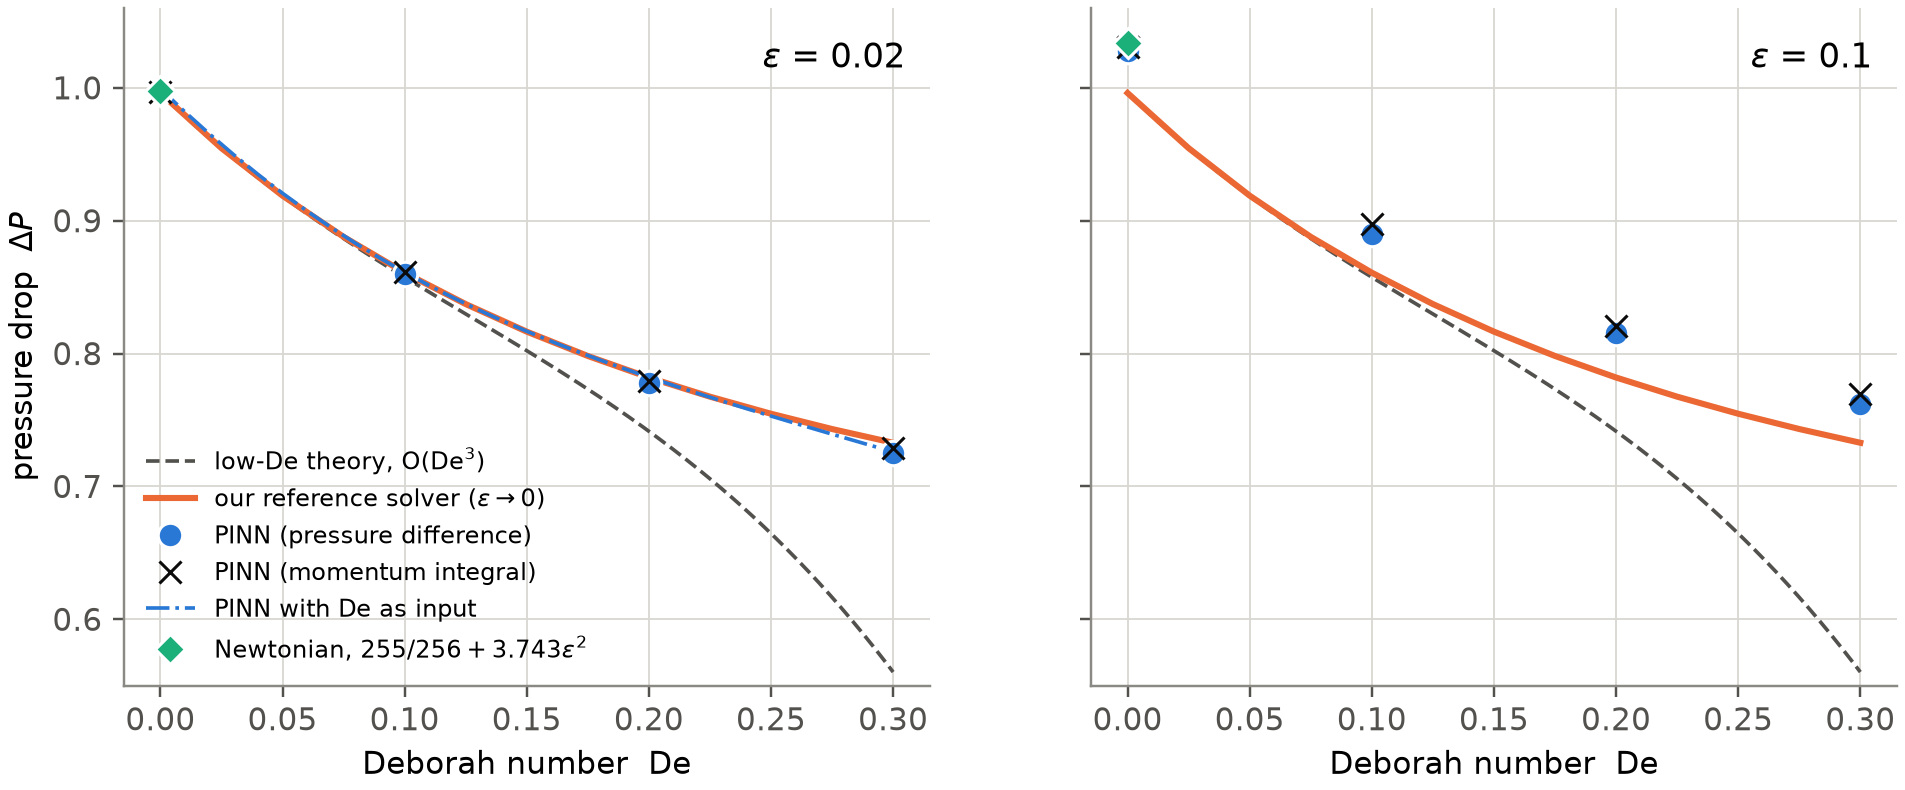
\includegraphics[width=\linewidth]{r06_dp_full2d.png}
\caption{Pressure drop against $\De$ for the full two-dimensional problem: $\epsilon=0.02$ (left) and $\epsilon=0.1$ (right). Circles: PINN, $\Delta P$ from the pressure (\ref{eq:dP}); crosses: PINN, $\Delta P$ from the momentum integral (\ref{eq:terms}); dash-dotted line: one PINN with $\De$ as input; solid line: reference solver for $\epsilon\to0$; dashed line: series (\ref{eq:series}); diamond: Newtonian estimate (\ref{eq:eps2}).}
\label{fig:dp2d}
\end{figure}

\subsection{Polymer stresses in the slender channel}
Figure~\ref{fig:stress} shows the PINN polymer stresses at $\epsilon=0.02$ for $\De=0.1$ and 0.3. Both components are near zero in the wide upstream part and build up in a wall layer that thickens and intensifies towards the outlet. The peak axial stress grows almost linearly with $\De$: $T_{zz}^{\max}=0.68$, 1.34 and 1.99 at $\De=0.1$, 0.2 and 0.3 (the $\epsilon\to0$ reference gives 0.70, 1.37 and 2.05, so the finite aspect ratio lowers the peak by about 3\,\%). A useful comparison is the fully developed value in a straight channel of the outlet height, $T_{zz}=18\bt\De=7.2\,\De$ at the wall, i.e.\ 0.72 and 2.16. The stress in the contraction stays below this value because the liquid arrives from a wider section where the shear rate was lower: with a memory time $\lambda$, the polymers have not had time to reach the stretch that the local shear rate would eventually produce. This lag is the essence of viscoelasticity and grows with $\De$ (5\,\% below the developed value at $\De=0.1$, 8\,\% at $\De=0.3$).

The shear stress behaves the opposite way: its most negative value, $-1.63$ ($\De=0.1$) and $-2.58$ ($\De=0.3$), is larger in magnitude than the Newtonian wall value at the outlet, $\bt\,\partial_YU_z=-3\bt=-1.2$. The first-order theory explains this. At $O(\De)$ the conformation contains $\tilde A_{yz,1}=-18H'Y(H^2-2Y^2)/H^7$, which at the outlet wall ($H=1$, $Y=1$, $H'=-0.75$) adds $\bt\De\times18H'=-0.54$ at $\De=0.1$, giving $-1.74$, close to the reference value $-1.69$. The extra shear stress is proportional to the wall slope $H'$: it exists only because the channel converges. (My symbolic derivation gives this expression with a minus sign; the arXiv version of the article prints it with a plus sign in its eq.\ (3.16b). The minus sign is the one consistent with the governing equations and with the PINN and reference fields.)

\begin{figure}[H]
\centering
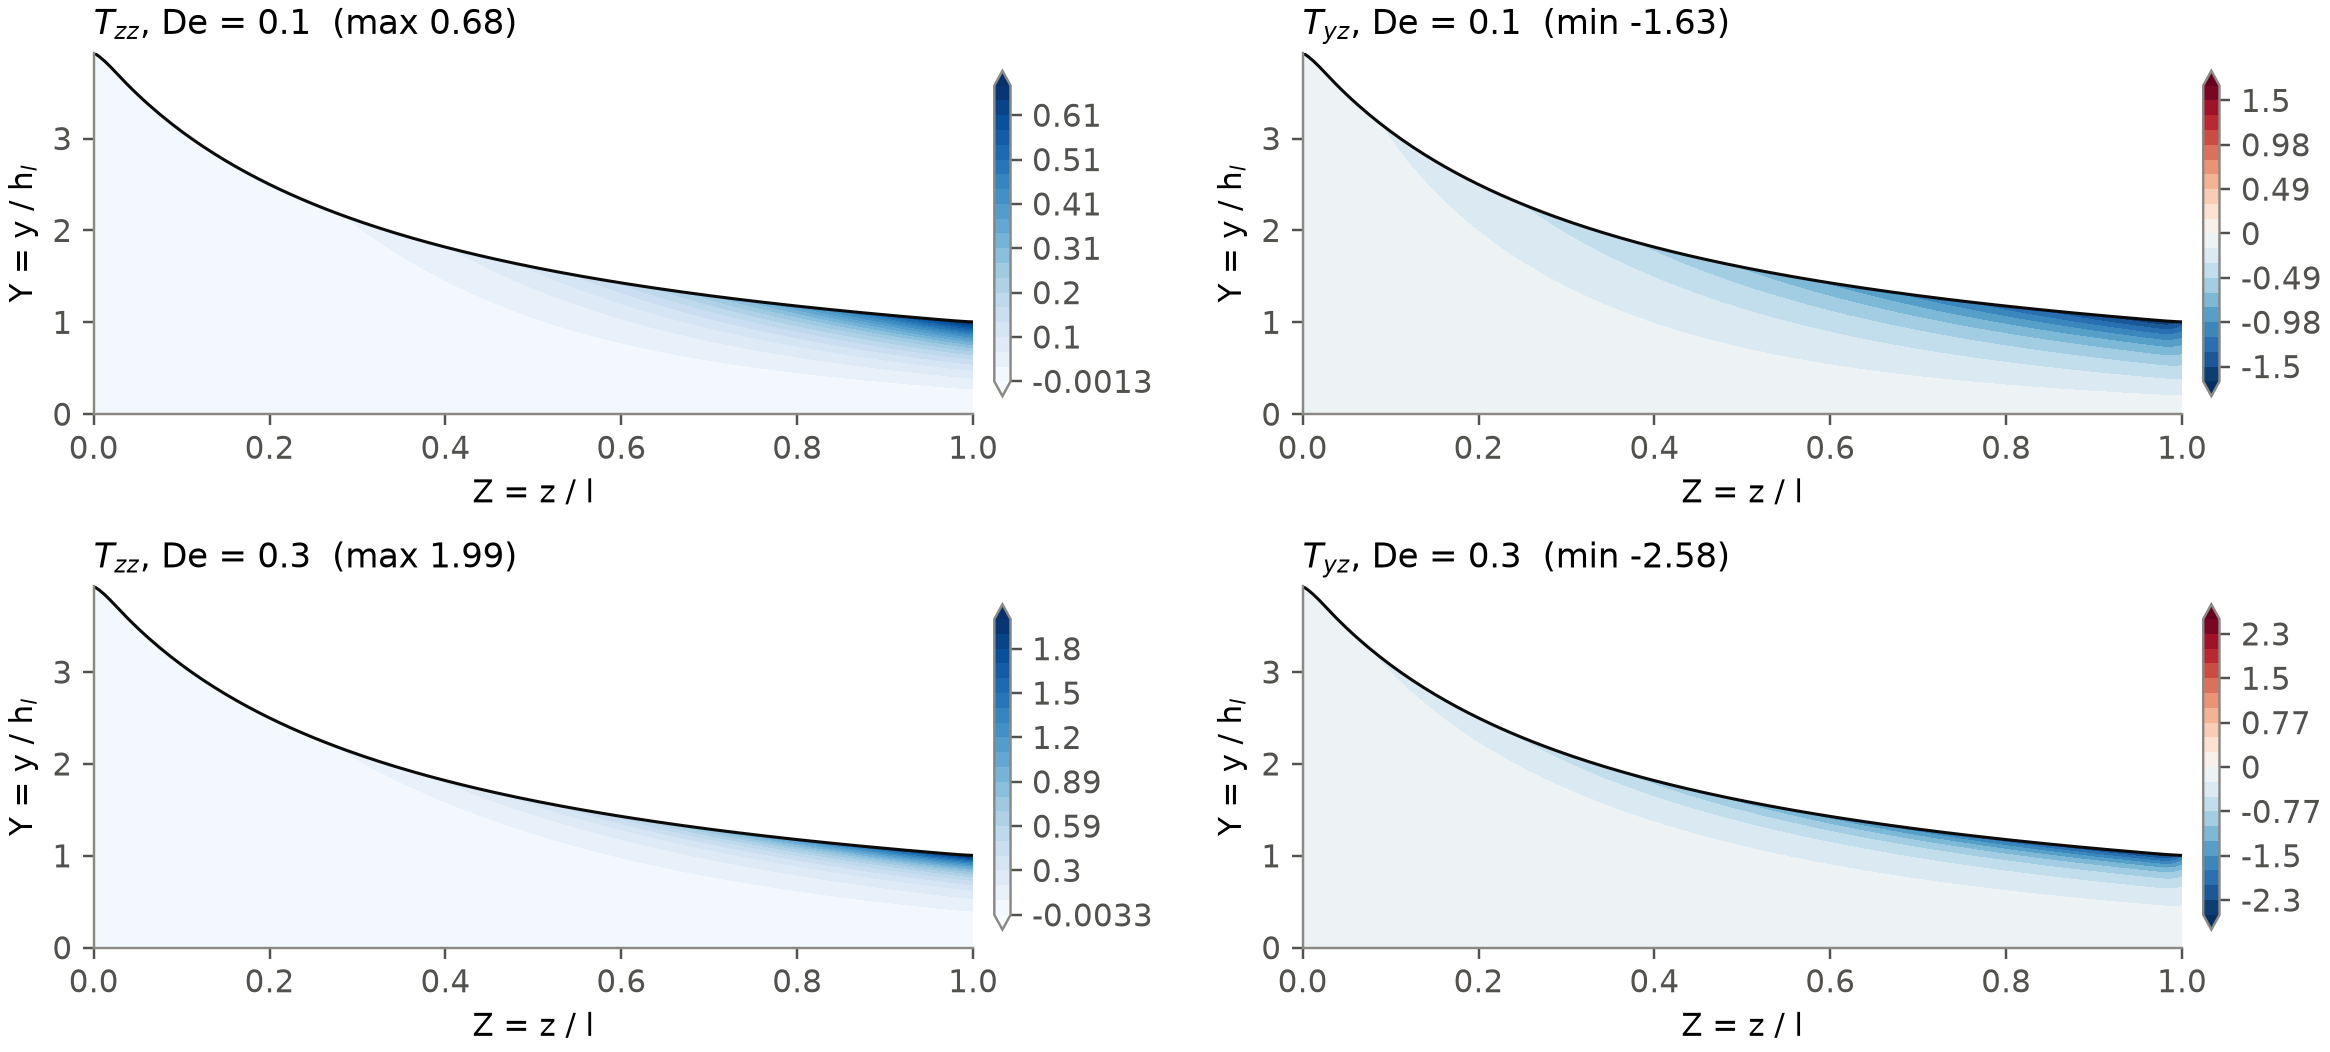
\includegraphics[width=\linewidth]{r07_stress_eps002.png}
\caption{PINN polymer stresses for the full two-dimensional problem at $\epsilon=0.02$: axial normal stress $T_{zz}$ (left) and shear stress $T_{yz}$ (right) at $\De=0.1$ (top) and $\De=0.3$ (bottom), over the contraction $0\le Z\le1$.}
\label{fig:stress}
\end{figure}

\subsection{Why elasticity lowers the pressure drop}
Figure~\ref{fig:contrib} shows the four contributions of (\ref{eq:terms}) against $\De$ for $\epsilon\to0$, where \term{1} vanishes. The viscous term \term{2} hardly changes, from 0.996 to 0.982 at $\De=0.3$, because the velocity profile on the centreline changes only slightly. The axial normal-stress term \term{3} is zero on the centreline: there is no shear on the axis, the inflow stress is zero there, and with $\epsilon\to0$ nothing creates axial stress on it. This is notable because $T_{zz}$ is the largest stress in the channel (figures~\ref{fig:fields} and \ref{fig:stress}), yet it lives near the wall and does not act on the centreline pressure. The whole reduction of $\Delta P$ comes from \term{4}, the gradient of the elastic shear stress, which grows from 0 to $-0.247$ at $\De=0.3$. The PINN reproduces each term (symbols), and the terms add up to the pressure drop within 0.3\,\%.

The physical picture is the following. As the channel narrows, the elastic shear stress near the centreline varies across the channel in a way that pushes the liquid forward, so less pressure gradient is needed for the same flow rate. The low-$\De$ theory (grey lines) captures this trend but, like the pressure-drop series, departs from the numerical result beyond $\De\approx0.15$. This decomposition agrees with the mechanism proposed in the article \cite{boyko2022}, now confirmed with an independent method up to $\De=0.3$.

\begin{figure}[H]
\centering
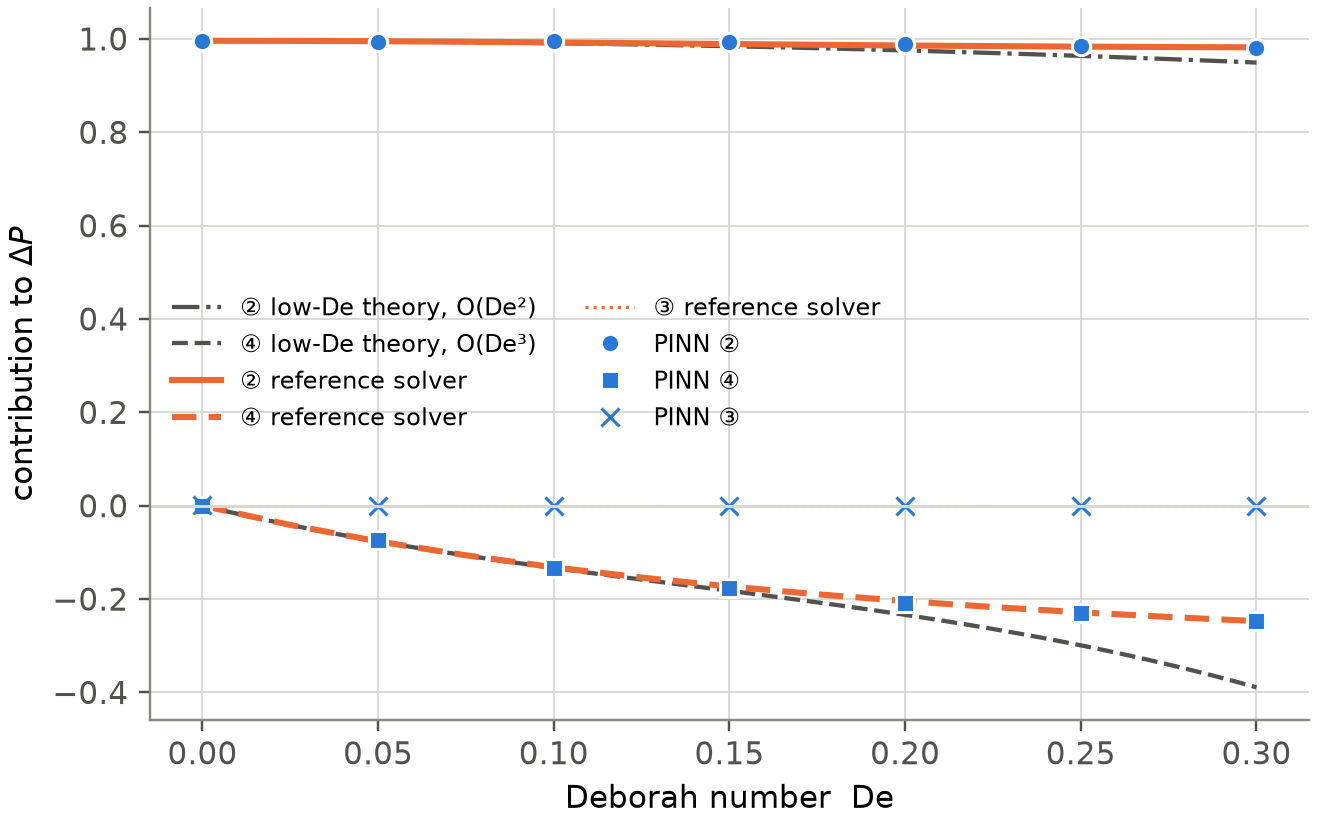
\includegraphics[width=0.66\linewidth]{r08_contributions.png}
\caption{Contributions to the centreline pressure drop, eq.~(\ref{eq:terms}), for $\epsilon\to0$: viscous term \term{2}, axial normal-stress term \term{3} and elastic shear-stress term \term{4}. Lines: reference solver; symbols: PINN; grey: low-$\De$ theory evaluated from the re-derived series.}
\label{fig:contrib}
\end{figure}

\subsection{Summary of the accuracy}
\begin{center}\footnotesize
\begin{tabular}{@{}lll@{}}
\toprule
Comparison & Result & Compared with\\
\midrule
PINN $\Delta P$, $\epsilon\to0$, $\De\le0.3$ & within 0.22\,\% (0.09\,\% momentum route) & reference solver\\
PINN fields, away from the corners & 0.01--0.5\,\% & reference solver\\
PINN fields, whole contraction, $\De=0.3$ & 0.2\,\% ($U_z$) to 2.1\,\% ($T_{zz}$) & reference solver\\
PINN $\Delta P$, $\epsilon=0.02$ and 0.1 & within 0.68\,\% & article's FE values (text only)\\
$\De$-input PINN, $\epsilon=0.02$ & within 0.6\,\% & fixed-$\De$ PINNs\\
Third-order series at $\De=0.3$ & 23.5\,\% too low & reference solver\\
\bottomrule
\end{tabular}
\end{center}

\section{Path forward}
\begin{itemize}
\item \textbf{Corners.} The remaining error sits at the two corners. Giving each corner zone its own sub-network (domain decomposition, as in XPINNs \cite{jagtap2020}), or adaptive sampling driven by the residual, should remove most of it.
\item \textbf{Higher elasticity.} The article and this work stop at $\De=0.3$. Continuation in $\De$ combined with the stress-layer scalings of Hinch \emph{et al.}\ \cite{hinch2024} could extend the PINN towards $\De\sim1$, where no closed-form result exists.
\item \textbf{A design tool.} A single network taking $\alpha$, $\bt$, $\epsilon$ and $\De$ as inputs would give the flow rate--pressure drop relation for a whole family of channels instantly, which is useful for designing microfluidic contractions.
\item \textbf{Inverse problem.} The same network can be trained to infer the relaxation time $\lambda$ from a measured $\Delta p$, turning the hyperbolic channel into a rheometer.
\item \textbf{Other models and shapes.} FENE-P or Giesekus fluids (bounded extensional stress) and the axisymmetric hyperbolic pipe \cite{housiadas2024} need only changes to the residuals.
\end{itemize}

\section{Conclusion}
\begin{itemize}
\item A physics-informed neural network with exact boundary conditions, exact flow rate and locally scaled residuals solves the steady Oldroyd-B flow in a 4:1 hyperbolic contraction for $0\le\De\le0.3$, both in the lubrication limit and in the full two-dimensional form, without any solution data.
\item Its pressure drop agrees with an independent reference solver within 0.22\,\% and with the article's finite-element results within 0.7\,\%; its fields agree within 0.01--0.5\,\% away from the corners.
\item Elasticity lowers the pressure drop by about 26\,\% at $\De=0.3$ for all three aspect ratios studied. The reduction comes entirely from the gradient of the elastic shear stress along the centreline; the axial normal stress, although the largest stress in the channel, does not act there.
\item The third-order low-$\De$ series is accurate only to $\De\approx0.1$ and is 23\,\% too low at $\De=0.3$, so a numerical solution is needed beyond that.
\item Marching the lubrication equations down the channel is ill-posed for $\De>0$; the problem has to be solved over the whole channel at once, which both the global Newton solver and the PINN do.
\end{itemize}

\section{Self-assessment}
I have reproduced the main results of the journal article (Level~1) with a method different from the one the authors used. Specifically, I reproduced the pressure drop as a function of the Deborah number for both channels studied in the article ($\epsilon=0.02$ and $0.1$, $0\le\De\le0.3$), with agreement within 0.7\,\% with the article's finite-element simulations; the qualitative structure of the polymer stress fields (positive axial stress and negative shear stress concentrated at the outlet wall); the failure of the third-order series beyond $\De\approx0.1$--$0.2$; and the article's explanation that the reduction of the pressure drop comes from the elastic shear-stress gradient. I did not reproduce the article's results on other contraction ratios $\alpha$ or viscosity ratios (its figures 7 and 8), and the PINN is least accurate, by a few percent, in small zones at the two corners. The most difficult parts were: making the PINN converge at all for a stiff, coupled system whose stresses vary 256-fold along the channel (solved by building every boundary condition into the network and scaling each residual by its local size); finding that the PINN pressure drop was 0.26\,\% wrong even with a small loss because the network let the pressure vary across the channel (solved by the pressure split in (\ref{eq:PA})); a first two-dimensional network that over-fitted at the inlet corner; and a reference solver that blew up until I understood that the problem is ill-posed for marching. Training on one laptop also limited how many variants I could test.

I do not claim new physics. The results of this work that go beyond reproduction (a partial Level~2) are methodological: (i) to my knowledge, the first PINN solution of this problem, including a single network valid for all $0\le\De\le0.3$; (ii) an independent global solver for the lubrication equations, together with the observation that marching them downstream is ill-posed for $\De>0$; (iii) the Newtonian aspect-ratio correction $\Delta P=255/256+3.743\,\epsilon^2$ for this channel; (iv) a sign error found in eq.~(3.16b) of the arXiv version of the article; and (v) a quantified statement of where the series stops being reliable. The physical mechanism itself is the one already given in the article.

\emph{Use of AI.} As stated in my project proposal, the literature search, code and text of this project were developed with the help of an AI assistant (Claude). I checked all results against the independent solver, the re-derived formulas and the article.

\begin{thebibliography}{99}\small
\setlength{\itemsep}{1pt}
\bibitem{alves2021} M.~A. Alves, P.~J. Oliveira and F.~T. Pinho (2021). Numerical methods for viscoelastic fluid flows. \emph{Annual Review of Fluid Mechanics} 53, 509--541.
\bibitem{bird1987} R.~B. Bird, R.~C. Armstrong and O. Hassager (1987). \emph{Dynamics of Polymeric Liquids, Vol.~1: Fluid Mechanics}, 2nd edn. Wiley, New York.
\bibitem{boyko2021} E. Boyko and H.~A. Stone (2021). Reciprocal theorem for calculating the flow rate--pressure drop relation for complex fluids in narrow geometries. \emph{Physical Review Fluids} 6, L081301.
\bibitem{boyko2022} E. Boyko and H.~A. Stone (2022). Pressure-driven flow of the viscoelastic Oldroyd-B fluid in narrow non-uniform geometries: analytical results and comparison with simulations. \emph{Journal of Fluid Mechanics} 936, A23. (arXiv:2109.06928.)
\bibitem{boyko2024} E. Boyko, E.~J. Hinch and H.~A. Stone (2024). Flow of an Oldroyd-B fluid in a slowly varying contraction: theoretical results for arbitrary values of Deborah number in the ultra-dilute limit. \emph{Journal of Fluid Mechanics} 988, A10.
\bibitem{christov2022} I.~C. Christov (2022). Soft hydraulics: from Newtonian to complex fluid flows through compliant conduits. \emph{Journal of Physics: Condensed Matter} 34, 063001.
\bibitem{curtis1974} A.~R. Curtis, M.~J.~D. Powell and J.~K. Reid (1974). On the estimation of sparse Jacobian matrices. \emph{IMA Journal of Applied Mathematics} 13, 117--119.
\bibitem{hinch2024} E.~J. Hinch, E. Boyko and H.~A. Stone (2024). Fast flow of an Oldroyd-B model fluid through a narrow slowly varying contraction. \emph{Journal of Fluid Mechanics} 988, A11.
\bibitem{housiadas2023} K.~D. Housiadas and A.~N. Beris (2023). Lubrication approximation of pressure-driven viscoelastic flow in a hyperbolic channel. \emph{Physics of Fluids} 35, 123116.
\bibitem{housiadas2024} K.~D. Housiadas and A.~N. Beris (2024). Pressure-driven viscoelastic flow in axisymmetric geometries with application to the hyperbolic pipe. \emph{Journal of Fluid Mechanics} 999, A7.
\bibitem{housiadas2025} K.~D. Housiadas (2025). An exact solution of the lubrication equations for the Oldroyd-B model in a hyperbolic channel. arXiv:2503.20636.
\bibitem{jagtap2020} A.~D. Jagtap and G.~E. Karniadakis (2020). Extended physics-informed neural networks (XPINNs): a generalized space-time domain decomposition based deep learning framework for nonlinear partial differential equations. \emph{Communications in Computational Physics} 28, 2002--2041.
\bibitem{karniadakis2021} G.~E. Karniadakis, I.~G. Kevrekidis, L. Lu, P. Perdikaris, S. Wang and L. Yang (2021). Physics-informed machine learning. \emph{Nature Reviews Physics} 3, 422--440.
\bibitem{kingma2015} D.~P. Kingma and J. Ba (2015). Adam: a method for stochastic optimization. \emph{International Conference on Learning Representations (ICLR)}.
\bibitem{krishnapriyan2021} A.~S. Krishnapriyan, A. Gholami, S. Zhe, R.~M. Kirby and M.~W. Mahoney (2021). Characterizing possible failure modes in physics-informed neural networks. \emph{Advances in Neural Information Processing Systems} 34, 26548--26560.
\bibitem{liu1989} D.~C. Liu and J. Nocedal (1989). On the limited memory BFGS method for large scale optimization. \emph{Mathematical Programming} 45, 503--528.
\bibitem{mahmoudabadbozchelou2022} M. Mahmoudabadbozchelou, G.~E. Karniadakis and S. Jamali (2022). nn-PINNs: non-Newtonian physics-informed neural networks for complex fluid modeling. \emph{Soft Matter} 18, 172--185.
\bibitem{matos2026} H.~M. Matos, C. Fernandes and M.~A. Alves (2026). Simulation of steady viscoelastic creeping flows with physics-informed neural networks. \emph{Journal of Non-Newtonian Fluid Mechanics} 350, 105637.
\bibitem{meurer2017} A. Meurer \emph{et al.} (2017). SymPy: symbolic computing in Python. \emph{PeerJ Computer Science} 3, e103.
\bibitem{oldroyd1950} J.~G. Oldroyd (1950). On the formulation of rheological equations of state. \emph{Proceedings of the Royal Society of London A} 200, 523--541.
\bibitem{oliveira2007} M.~S.~N. Oliveira, M.~A. Alves, F.~T. Pinho and G.~H. McKinley (2007). Viscous flow through microfabricated hyperbolic contractions. \emph{Experiments in Fluids} 43, 437--451.
\bibitem{paszke2019} A. Paszke \emph{et al.} (2019). PyTorch: an imperative style, high-performance deep learning library. \emph{Advances in Neural Information Processing Systems} 32, 8024--8035.
\bibitem{raissi2019} M. Raissi, P. Perdikaris and G.~E. Karniadakis (2019). Physics-informed neural networks: a deep learning framework for solving forward and inverse problems involving nonlinear partial differential equations. \emph{Journal of Computational Physics} 378, 686--707.
\bibitem{rao2020} C. Rao, H. Sun and Y. Liu (2020). Physics-informed deep learning for incompressible laminar flows. \emph{Theoretical and Applied Mechanics Letters} 10, 207--212.
\bibitem{sialmas2025} P. Sialmas and K.~D. Housiadas (2025). General evaluation of the pressure gradient for lubrication flows in varying channels with applications to linear and hyperbolic contractions. \emph{Journal of Non-Newtonian Fluid Mechanics} 346, 105487.
\bibitem{sukumar2022} N. Sukumar and A. Srivastava (2022). Exact imposition of boundary conditions with distance functions in physics-informed deep neural networks. \emph{Computer Methods in Applied Mechanics and Engineering} 389, 114333.
\bibitem{tavakol2017} B. Tavakol, G. Froehlicher, D.~P. Holmes and H.~A. Stone (2017). Extended lubrication theory: improved estimates of flow in channels with variable geometry. \emph{Proceedings of the Royal Society A} 473, 20170234.
\bibitem{thakur2024} S. Thakur, M. Raissi and A.~M. Ardekani (2024). ViscoelasticNet: a physics informed neural network framework for stress discovery and model selection. \emph{Journal of Non-Newtonian Fluid Mechanics} 330, 105265.
\bibitem{trefethen2000} L.~N. Trefethen (2000). \emph{Spectral Methods in MATLAB}. SIAM, Philadelphia.
\bibitem{wang2021grad} S. Wang, Y. Teng and P. Perdikaris (2021). Understanding and mitigating gradient flow pathologies in physics-informed neural networks. \emph{SIAM Journal on Scientific Computing} 43, A3055--A3081.
\bibitem{wang2023guide} S. Wang, S. Sankaran, H. Wang and P. Perdikaris (2023). An expert's guide to training physics-informed neural networks. arXiv:2308.08468.
\end{thebibliography}

\end{document}
